\documentclass{article}
\usepackage{cancel}
\usepackage[utf8]{inputenc}
\usepackage {titlesec}
\usepackage[english,russian]{babel}
\usepackage{amssymb}
\usepackage{amsmath}
\usepackage{wasysym}
\usepackage{graphicx}
\usepackage{numprint}
\graphicspath{{pictures/}}

\titlespacing*{\section}{\parindent}{*4}{*4}

\title{Домашнее задание 15}
\author{Ткачев Андрей, группа 166}
\date{\today}
\newcommand{\niton}{\not\owns}
\newcommand{\pr}{^{\prime}}
\newcommand{\ppr}{^{\prime\prime}}
\newcommand{\xp}{x^{\prime}}
\newcommand{\xpp}{x^{\prime\prime}}
\newcommand{\xppp}{x^{\prime\prime\prime}}
\newcommand{\pair}[2]{(#1,\ #2)}
\newcommand{\andi}{$ и $}
\newcommand{\half}[1]{\frac{#1}{2}}
\newcommand{\eqp}{\sim}
\newcommand{\N}{\mathbb{N}}
\newcommand{\R}{\mathbb{R}}
\newcommand{\Q}{\mathbb{Q}}

\begin{document}
    \maketitle
    \paragraph{Задача 1.}
    Пусть $S$ -- множество кругов на плосткости. Поймем, что существует биекция $f: S \rightarrow \R \times \R \times \R_+$. Действительно, каждый круг однозначно определяется координатами центра и радиусом. Т.е. каждому кругу в однозначное соответствие можно поставить три вещественных числа $(r_0, r_1, r_2)$, где $\pair{r_0}{r_1}$ определяет центр, а $r_2$ -- радиус ($r_2 > 0$). При этом, раз ничего не сказано про персечения, то можно считать, что такие $(r_0, r_1, r_2)$ всегда задают какой-то круг. 

    Так как $\R_+ \sim \R$, то $\R \times \R \times \R_+  \sim \R \times \R \times \R \sim \R$. Но тогда $S \sim \R$. Значит $S$ -- континуально.

    \paragraph{Задача 2.}
    Нет не верно. Например на плоскости можно отметить континуум окружностей, имеющих общий центр (каждая окружность в этом случае задается лишь одним числом -- радиусом $r \in \R_+$, т.е. их действительно будет континуум). Но множество центров этих окружностей -- конечно (состоит из единственного элемента).

    \paragraph{Задача 3.}
    Да, существует. Возьмем множество $\R \times \R$. Для каждого $r_0 \in \R$ заведем подмножество в $\R \times \R$ в которое входят все пары вида $\pair{r_0}{r}$, $r \in \R$. Поймем, что все такие подмножества не пересекаются в силу различия первых элементов в парах, их образующих, и что всего таких подмножеств столько же, сколько и вариантов первого числа в паре, т.е. континуум.

    Вспомним, что $\R \times \R \sim \R$, а значит существует биекция $f: \R \times \R \rightarrow \R$. Но тогда, у каждого из построенных нами подмножеств в $\R \times \R$ существует образ в $\R$, причем, в силу биективности отображения, эти образы не пересекаются и их ровно столько же, сколько и их прообразов в $\R \times \R$, а значит континуум.

    \paragraph{Задача 4.}
    Нет, не верно. Рассмотрим, например множество $S$ функий $f: \N \rightarrow \{0, 1\}$. Т.е. каждая такая функция взаимно однозначно задает бесконечную двоичную последовательность. Значит число таких функций равно числу бесконечных двоичных последоваетельностей, которых как мы знаем -- континуум (Вообще, $S$ в данном случае -- ни что иное, как $2^{\N}$).

    \paragraph{Задача 5.}
    Да, верно. Пусть множество двоичных последовательностей без трех единиц подряд -- $S$. Покажем что существует биекция между $2^{\N}$ и $S$.

    Заметим, что $S \apprle 2^{\N}$. Инъекция в этом случае очевидна: каждой последовательности из $S$ поставим в соответствие ее же саму в $2^{\N}$.

    Покажем, что $2^{\N} \apprle S$. Поймем, что любую последовательность из $2^{\N}$ можно разбить на <<блоки>> по два символа, начиная с первого ($10001101\ldots \rightarrow 10\ 00\ 11\ 01\ \ldots$). Сопоставим каждому такому блоку код, которым мы будем его заменять, для получения последоваетльности из $S$.

    \begin{itemize}
        \item $00 \rightarrow 000$
        \item $01 \rightarrow 001$
        \item $10 \rightarrow 100$
        \item $11 \rightarrow 010$
    \end{itemize}

    Т.е. для каждой строки из $2^{\N}$ мы, по указанному правилу, сможем сопоставить некоторую бесконечную двоичную строку, причем разным строкам сопоставятся разные (если начальные строки различались в $i$-ом блоке, то конечные будут различатся в $i$-ом триплете). Поймем, что эта некоторая бесконечная двоичная строка удовлетворяет требованиям задачи, а именно не содержит трех единиц подряд (никакая комбинация из указанных триплетов не даст больше чем две подряд стоящие единицы). Значит мы получили инъекцию $2^{\N} \rightarrow S$.

    Тогда, по теореме Кантора-Бейрштейна существует биекция $S \leftrightarrow 2^{\N}$, а значит $S \sim 2^{\N}$. Получаем, что $S$ имеет мощность конитинуум.

    \paragraph{Задача 6.}
    Будем отождествлять в данной задаче множество функций из $\N$ в абстрактное множество $A$ и бесконечные последовательности состоящие из элементов $A$, которыми функция и определяется.

    Множество биективных функций $\N \rightarrow \N$ (а значит и множество бесконечных последовательностей натуральных, в которых ни одно оне повторяется дважлы) будем обозначать, как $\N_b^{\N}$.

    Покажем, что $\N_b^{\N}$ не больше, чем континуум. Действительно, $\N_b^{\N} \subseteq \N^{\N} \sim 2^{\N}$. Тогда $\N_b^{\N} \apprle \N^{\N}$, а значит, не больше континуума.

    Докажем теперь, что $2^{\N} \apprle \N_b^{\N}$. Сопоставим каждой двоичной последовательности свою последовательность из натуральных чисел, в которой ни какое число не встречается дважды, по следующему правилу:

    \begin{itemize}
        \item Если $i$-ый бит равен 0, то в результирующей последовательности на позиции $2i \andi 2i + 1$ поставим $2i \andi 2i + 1$ соответвенно.

        \item Если $i$-ый бит равен 1, то в результирующей последовательности на позиции $2i \andi 2i + 1$ поставим $2i + 1 \andi 2i$ соответвенно.
    \end{itemize}

    Так например, последовательности $10\ldots$ будет соответсвовать $1, 0, 2, 3, \ldots$.

    Поймем, что это отображение инъективно -- если исходные последовательности различаются в $i-$ом бите, то конечные последовательности отличаются в числе с номером $2i$. Причем, эта конечная последовательность входит в $\N_b^{\N}$ (если сопоставить каждому члену бесконечной последовательности из $\N^{\N}$ соответсвующий член в полученной, то получится биекция).

    Таким образом, $2^{\N} \apprle \N_b^{\N}$. 

    Тогда, по теореме Кантора-Берштейна $2^{\N} \sim \N_b^{\N}$, значит $\N_b^{\N}$ -- континуально.

    \paragraph{Задача 7.}
    Разместим на плоскости континуум <<единиц>>. Возьмем, и разместим на плоскости одну единицу. Проведем биссектриссу ее угла. Теперь параллельным переносом вдоль этой прямой мы можем <<скопировать>> уже существующую единицу на любом расстоянии от нее. Тогда мы можем каждому вещественному числу $r$ сопоставить <<единицу>> на плоскости, вершина угла которой удалена от начальной вершины ровно на $r$ (полученные единицы не будут пересекаться, т.е. прямые, которые их образуют -- параллельны по построению). Таким образом существует биекция между вещественными числами и <<единицами>> на плоскости, а значит фигурок -- континуум.

    \paragraph{Задача 8.}
    Рассмотрим какую-либо окружнось.

    Покажем, что в ней мы можем выбрать точку с рациональными координатами (См. рисунок и абзац ниже).

    \begin{center}
    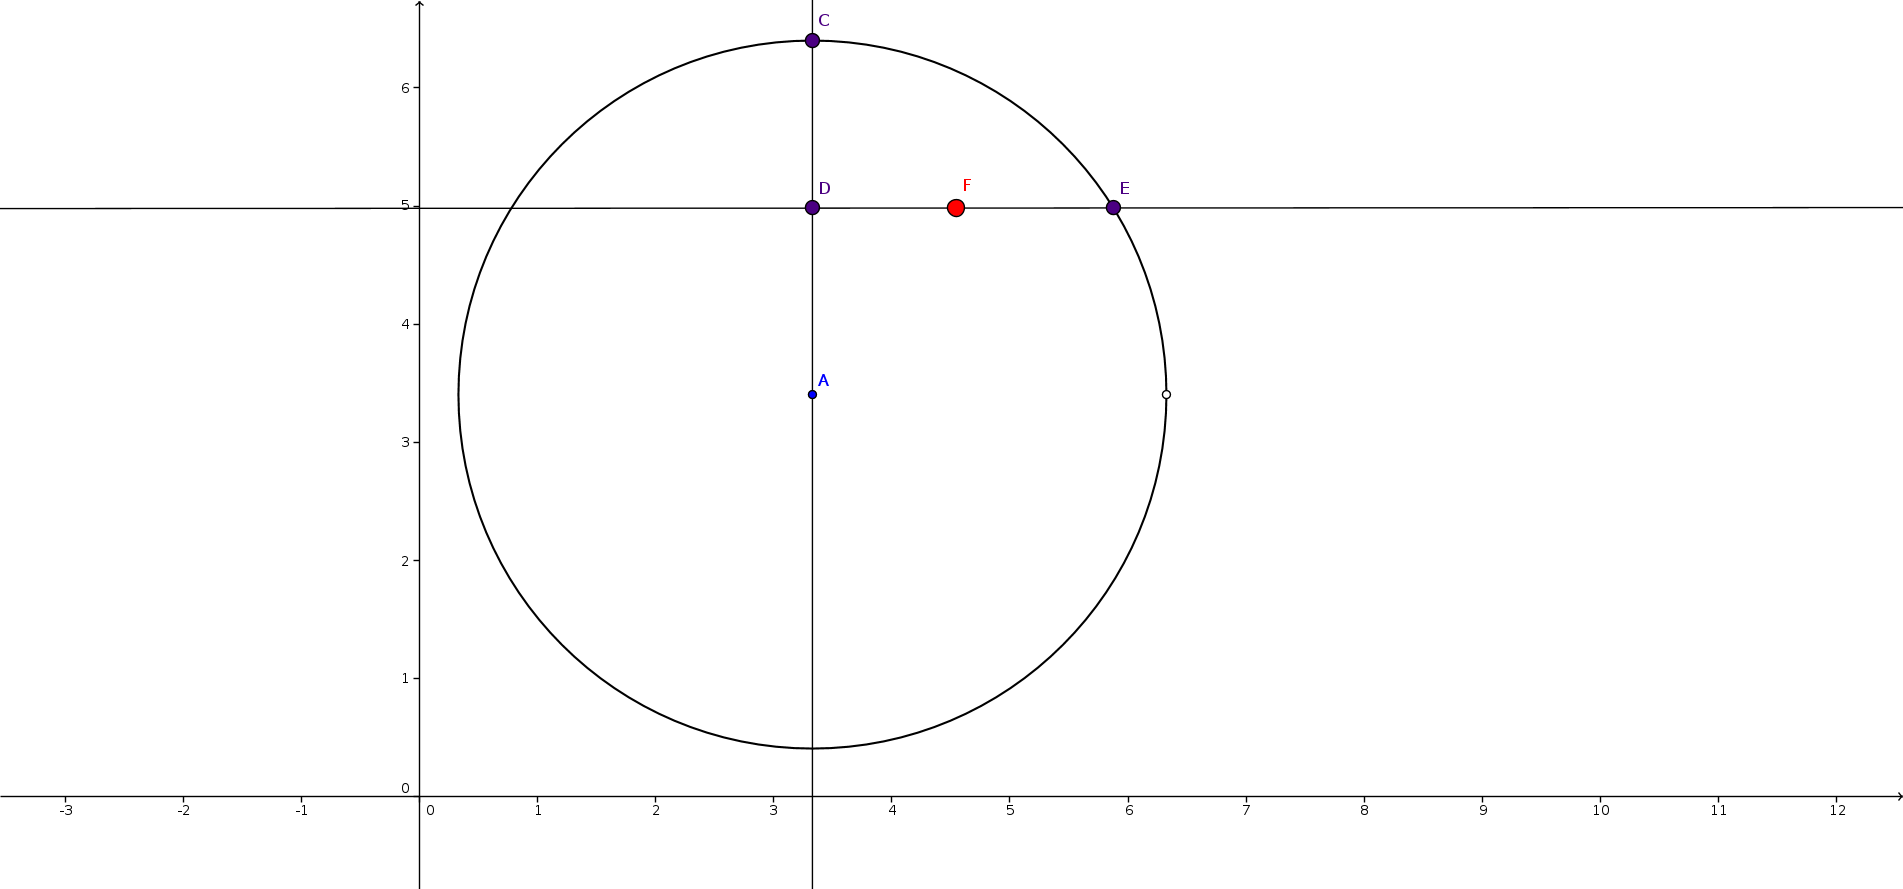
\includegraphics[scale=0.8]{8_1}
    \end{center}

    Для этого, проведем через центр прямую $AC$ параллельную оси ординат. На отрезке $AC$ выберем точку $D$ с целочисленной ординатой (Например с ординатой равной среднему арифметическому ординат $A$ и $C$ взятых с избытком и с недостатком). 
    Через нее проведем прямую параллельно оси абсцисс и на отрезке $DE$ выбереме точку с рациональной абсциссой (аналогично, как и в прошлый раз). Эта точка - искомая, так как ее координаты рациональны.

    Отлично, теперь мы умеем однозначно(односторонняя однозначность) сопоставлять каждой окружности рациональную точку, находящуюся в ее пределах.

    Пусть у нас имеется плоскость с бесконечным числом непресесекающихся восьмерок. Сопоставим каждой из них две рациональные точки - по рациональной точке на каждую из окружностей, образующих восьмерку. Заметим, что никакие две пары точек не совпадают (иначе, мы бы имели две пересекающиеся хотябы в одной точке восьмерки, т.к. двум окружностям споставляется одна и таже рац. точка, если центр одной из них находится в другой; значит мы имеем восьмерки, ни одна из которых не лежит полностью в окружности другой и не лежит во вне, а значит они как-то пересекаются).

    Значит мы построили инъекцию из множества восьмерок в $\Q \times \Q \sim \N$. Таким образом множество восьмерок не более чем счетно.

\end{document}